% Options for packages loaded elsewhere
\PassOptionsToPackage{unicode}{hyperref}
\PassOptionsToPackage{hyphens}{url}
\documentclass[
]{article}
\usepackage{xcolor}
\usepackage{amsmath,amssymb}
\setcounter{secnumdepth}{-\maxdimen} % remove section numbering
\usepackage{iftex}
\ifPDFTeX
  \usepackage[T1]{fontenc}
  \usepackage[utf8]{inputenc}
  \usepackage{textcomp} % provide euro and other symbols
\else % if luatex or xetex
  \usepackage{unicode-math} % this also loads fontspec
  \defaultfontfeatures{Scale=MatchLowercase}
  \defaultfontfeatures[\rmfamily]{Ligatures=TeX,Scale=1}
\fi
\usepackage{lmodern}
\ifPDFTeX\else
  % xetex/luatex font selection
\fi
% Use upquote if available, for straight quotes in verbatim environments
\IfFileExists{upquote.sty}{\usepackage{upquote}}{}
\IfFileExists{microtype.sty}{% use microtype if available
  \usepackage[]{microtype}
  \UseMicrotypeSet[protrusion]{basicmath} % disable protrusion for tt fonts
}{}
\makeatletter
\@ifundefined{KOMAClassName}{% if non-KOMA class
  \IfFileExists{parskip.sty}{%
    \usepackage{parskip}
  }{% else
    \setlength{\parindent}{0pt}
    \setlength{\parskip}{6pt plus 2pt minus 1pt}}
}{% if KOMA class
  \KOMAoptions{parskip=half}}
\makeatother
\usepackage{longtable,booktabs,array}
\usepackage{calc} % for calculating minipage widths
% Correct order of tables after \paragraph or \subparagraph
\usepackage{etoolbox}
\makeatletter
\patchcmd\longtable{\par}{\if@noskipsec\mbox{}\fi\par}{}{}
\makeatother
% Allow footnotes in longtable head/foot
\IfFileExists{footnotehyper.sty}{\usepackage{footnotehyper}}{\usepackage{footnote}}
\makesavenoteenv{longtable}
\usepackage{graphicx}
\makeatletter
\newsavebox\pandoc@box
\newcommand*\pandocbounded[1]{% scales image to fit in text height/width
  \sbox\pandoc@box{#1}%
  \Gscale@div\@tempa{\textheight}{\dimexpr\ht\pandoc@box+\dp\pandoc@box\relax}%
  \Gscale@div\@tempb{\linewidth}{\wd\pandoc@box}%
  \ifdim\@tempb\p@<\@tempa\p@\let\@tempa\@tempb\fi% select the smaller of both
  \ifdim\@tempa\p@<\p@\scalebox{\@tempa}{\usebox\pandoc@box}%
  \else\usebox{\pandoc@box}%
  \fi%
}
% Set default figure placement to htbp
\def\fps@figure{htbp}
\makeatother
\ifLuaTeX
  \usepackage{luacolor}
  \usepackage[soul]{lua-ul}
\else
  \usepackage{soul}
\fi
\setlength{\emergencystretch}{3em} % prevent overfull lines
\providecommand{\tightlist}{%
  \setlength{\itemsep}{0pt}\setlength{\parskip}{0pt}}
\usepackage{bookmark}
\IfFileExists{xurl.sty}{\usepackage{xurl}}{} % add URL line breaks if available
\urlstyle{same}
\hypersetup{
  hidelinks,
  pdfcreator={LaTeX via pandoc}}

\author{}
\date{}

\begin{document}

\textbf{TÍTULO DO TRABALHO}

\textbf{Primeiro Autor\textsuperscript{1}, Segundo
Autor\textsuperscript{2}, Terceiro Autor\textsuperscript{1,2}}

\begin{quote}
\emph{\textsuperscript{1}Afiliação institucional do primeiro autor,
Cidade, País (e-mail do autor principal)}

\emph{\textsuperscript{2}Afiliação institucional do segundo autor,
Cidade, País}

\emph{Resumo:}~O resumo deve conter no máximo 500 caracteres incluindo
os espaços o resumo deve conter no máximo 500 caracteres incluindo os
espaços o resumo deve conter no máximo 500 caracteres incluindo os
espaços o resumo deve conter no máximo 500 caracteres incluindo os
espaços o resumo deve conter no máximo 500 caracteres incluindo os
espaços o resumo deve conter no máximo 500 caracteres incluindo os
espaços o resumo deve conter no máximo 500 caracteres incluindo os
espaços o resumo deve conter no máximo 500 caracteres incluindo os
espaços.

\emph{Palavras-chave}:\textbf{~}Digite as palavras-chaves separadas por
ponto e vírgula (;), máximo 5 palavras-chave
\end{quote}

INTRODUÇÃO

Este documento irá auxiliá-lo a preparar o seu trabalho (\ul{máximo 5
páginas}) para os Anais do CoBICET. Todas as instruções para layout,
estilo e escrita do trabalho são fornecidas. Nós encorajamos você a
salvar este documento com um nome diferente, excluir todo o texto e usar
o mesmo documento em branco para escrever o seu trabalho. O template
contém todos os estilos necessários e está pronto para ser utilizado.
Use o estilo de parágrafo, tal como definido neste documento. Não
incluir números de página ou qualquer outro cabeçalho ou rodapé de
página.

O trabalho deverá conter: Resumo, Palavras-chave, Introdução, Material e
Métodos, Resultados e Discussão, Conclusão, Agradecimentos (se houver) e
Referências.

O texto da introdução deverá contemplar uma pequena revisão sobre a
temática na qual o trabalho está inserido. Deverá ainda apresentar o
contexto geral do trabalho. Ao final da introdução indicar de forma
sucinta os principais objetivos a serem atendidos pelo trabalho.

MATERIAL E MÉTODOS

As metodologias utilizadas no trabalho para atingir os objetivos
propostos deverão ser explicadas sucintamente.

RESULTADOS E DISCUSSÃO

Apresentar os resultados obtidos no trabalho e sua discussão em relação
ao conhecimento já disponível. Nos resultados poderão ser apresentadas
tabelas, gráficos e outras ilustrações que sejam essenciais à boa
compreensão do texto.

Figuras: Por favor, use figuras de boa qualidade (fotografias, gráficos)
e coloridas, pois os anais do evento serão fornecidos de forma
eletrônica.

As Figuras devem ser numeradas e centradas (ver Figura 1). Por favor,
tome cuidado para que o título fique logo abaixo da figura (e não na
próxima coluna).

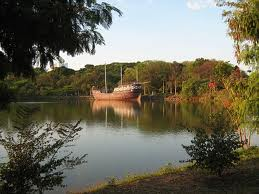
\includegraphics[width=1.53611in,height=1.14514in,alt={taquaral2}]{imagens/media/image2.jpeg}

Figura~1. Título da figura.

Tabelas: As tabelas podem ser inseridas no texto sendo enumeradas de
acordo com a sequência. O título da tabela deve estar alinhado à
esquerda.

Tabela 1. Título da tabela.

\begin{longtable}[]{@{}
  >{\raggedright\arraybackslash}p{(\linewidth - 2\tabcolsep) * \real{0.6000}}
  >{\centering\arraybackslash}p{(\linewidth - 2\tabcolsep) * \real{0.4000}}@{}}
\toprule\noalign{}
\begin{minipage}[b]{\linewidth}\raggedright
Atividades
\end{minipage} & \begin{minipage}[b]{\linewidth}\centering
Datas importantes
\end{minipage} \\
\midrule\noalign{}
\endhead
\bottomrule\noalign{}
\endlastfoot
Início das submissões dos trabalhos & Aberto \\
Parecer final do comitê científico & Consultar site \\
\end{longtable}

Equações devem estar centralizadas e numeradas na sequência (exemplo
abaixo):

\pandocbounded{\includegraphics[keepaspectratio]{imagens/media/image3.wmf}}
(1)

Citações no texto: Quando uma publicação é citada no texto, acrescente o
nome do autor(es) e o ano da publicação dentro de parênteses: (Mujumdar,
1990). Para dois autores: (Farkas e Rendik, 1997). Para três ou mais
autores: (Pelissari et al., 2014).

Para citações diretas, apenas colocar o ano entre parênteses, Por
exemplo: ``De acordo com Pelissari et al. (2013), as ...''.

CONCLUSÃO

Indicar de forma objetiva as principais conclusões obtidas pelo
trabalho.

O trabalho não será reformatado, por isso, siga rigorosamente as
instruções dadas acima, caso contrário ele poderá ser recusado ou
devolvido para melhoria.

AGRADECIMENTOS

Escreva os agradecimentos aqui.

REFERÊNCIAS

A lista de referências devem ser organizada em ordem alfabética de
acordo com o primeiro autor. Não enumere as referências. Publicações do
mesmo autor(es) deverão estar listadas em ordem de acordo com o ano de
publicação. No caso de mais de uma publicação por autor no mesmo ano,
colocar letras a, b, c, etc. e ano (2006a). Por favor, note que todas as
referências listadas aqui devem estar citadas no corpo do texto.

Autor(es) do livro. Título do livro. (Nome do editor(es)). Editora,
Lugar da publicação, Ano.

Autor(es) da revista. Título do artigo. Nome da revista, volume, número
das páginas, Ano.

\end{document}
